%----------------------------------------------------------------------------------------
%	PACKAGES AND THEMES
%----------------------------------------------------------------------------------------
\documentclass[aspectratio=169,xcolor=dvipsnames,handout]{beamer}
\usetheme{Darmstadt}
\usecolortheme{seahorse}

\usepackage[hangul]{kotex}
\usepackage{hyperref}
\usepackage{graphicx} % Allows including images
\usepackage{booktabs, multicol, multirow} % Allows the use of \toprule, \midrule and \bottomrule in tables
\setbeamercovered{transparent}
\addtocontents{toc}{\setcounter{tocdepth}{2}} 
%----------------------------------------------------------------------------------------
%	TITLE PAGE
%----------------------------------------------------------------------------------------

\title[생산성과 불평등]{생산성과 불평등} % The short title appears at the bottom of every slide, the full title is only on the title page
\subtitle{경제정의와 불평등}

\author[오성재]{오성재}

\institute[HNU] % Your institution as it will appear on the bottom of every slide, may be shorthand to save space
{
    한남대학교 \\
    탈메이지 교양학부 \\
}
\date{\today} % Date, can be changed to a custom date


%--------------------------------------------------------------------
%	PRESENTATION SLIDES
%--------------------------------------------------------------------

\begin{document}

\begin{frame}
    \titlepage
\end{frame}

\begin{frame}{목차}
    \tableofcontents
\end{frame}
%------------------------------------------------

%------------------------------------------------
\section{생산성의 역설}

\begin{frame}{}
    \begin{itemize}
        \item 최근 수십 년 동안 생산성 성장이 지속적이고 걱정스러울 정도로 둔화.
        \begin{itemize}
            \item 최근의 경기 침체는 영구적인 현상이라는 비관론.
            \item 반대로, 기술 낙관론자들은 기술 발전의 기본 속도가 느려지지 않았으며 IT 혁명이 계속해서 국경 경제를 극적으로 변화시킬 것.
        \end{itemize}
    \end{itemize}
\end{frame}
%------------------------------------------------

\subsection{총노동생산성 추이}

\begin{frame}{}
    \begin{itemize}
        \item  생산성은 "더 열심히 일하는 것"이 아니라 "더 똑똑하게 일하는 것"에 관한 것.
    \end{itemize}
\end{frame}
%------------------------------------------------

\subsubsection{ 생산성 향상은 대부분의 선진국에서 최근 수십 년 동안 감소하고 }

\begin{frame}{}
    \begin{itemize}
        \item 1990년대 중반까지 선진국의 총 노동 생산성 증가는 생산성 경계로의 수렴에 의해 주도. 
    \end{itemize}
    \begin{figure}
        \centering
        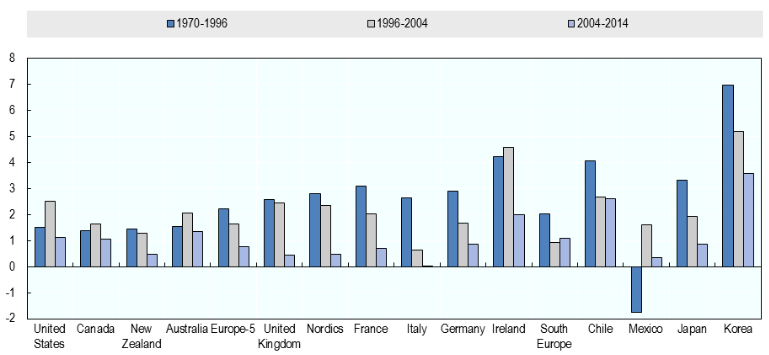
\includegraphics[scale=.4]{pic/tpin1.1.png}
        \caption{국가별 단위시간당 GDP의 연평균 성장률}
    \end{figure}
\end{frame}
%------------------------------------------------

\begin{frame}{}
    \begin{itemize}
        \item 수렴 과정은 1990년대 중반에 약화되었고, 다수의 OECD 국가에서 총 노동 생산성 증가가 둔화.
    \end{itemize}
    \begin{figure}
        \centering
        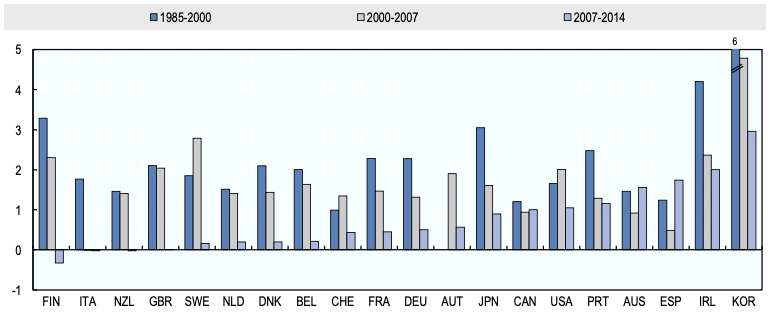
\includegraphics[scale=.4]{pic/tpin1.2.1.png}
        \caption{국가별 노동생산성의 성장률}
    \end{figure}
\end{frame}
%------------------------------------------------

\begin{frame}{}
    \begin{itemize}
        \item 같은 기간 자본의 생산성은 소폭 하락.
    \end{itemize}
    \begin{figure}
        \centering
        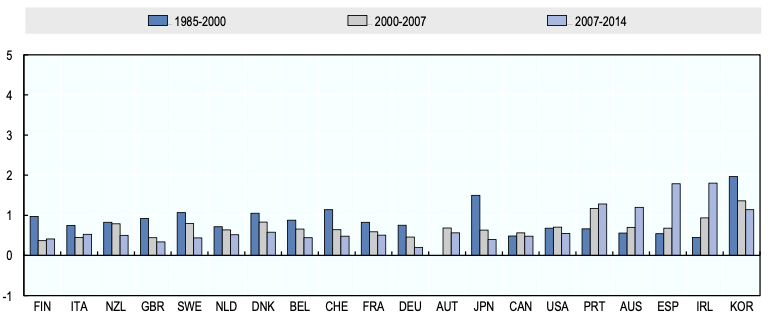
\includegraphics[scale=.4]{pic/tpin1.2.2.png}
        \caption{국가별 자본심화의 기여분}
    \end{figure}
\end{frame}
%------------------------------------------------

\begin{frame}{}
    \begin{itemize}
        \item 수렴 과정 약화의 일부분은 총요소 생산성의 하락으로도 설명 가능.
    \end{itemize}
    \begin{figure}
        \centering
        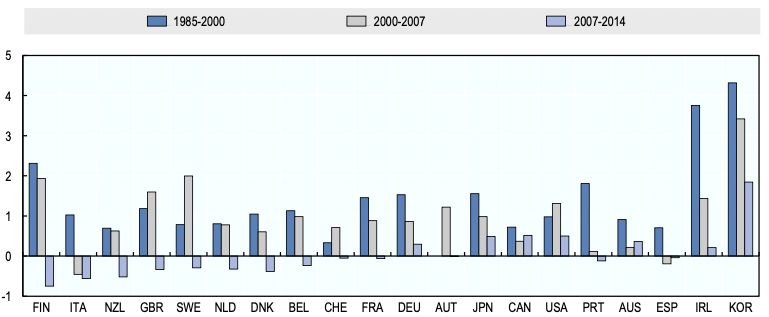
\includegraphics[scale=.4]{pic/tpin1.2.3.png}
        \caption{국가별 요소생산성의 성장률}
    \end{figure}
\end{frame}
%------------------------------------------------

\subsubsection{ 신흥국과 개발도상국은 OECD 국가를 충분히 빠르게 따라가지 못했으며 현재 생산성도 저하}


\begin{frame}{}
    \begin{itemize}
        \item 신흥국과 개발도상국의 노동 생산성 수준은 계속해서 선진국보다 훨씬 낮음.
    \end{itemize}
    \begin{figure}
        \centering
        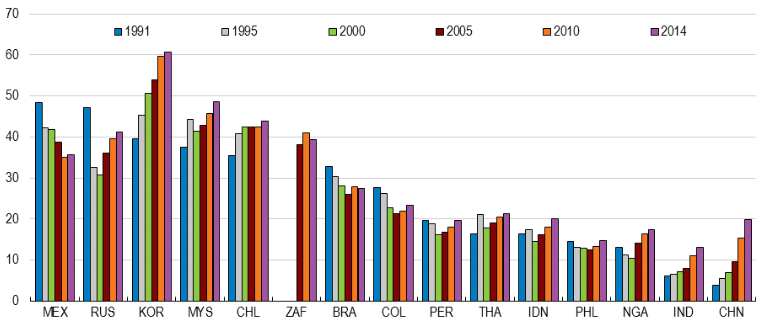
\includegraphics[scale=.3]{pic/tpin1.3.png}
        \caption{미국 대비 노동생산성}
    \end{figure}
\end{frame}
%------------------------------------------------

\begin{frame}{}
    \begin{itemize}
        \item 금융위기 이후 신흥국의 총요소생산성은 둔화.
    \end{itemize}
    \begin{figure}
        \centering
        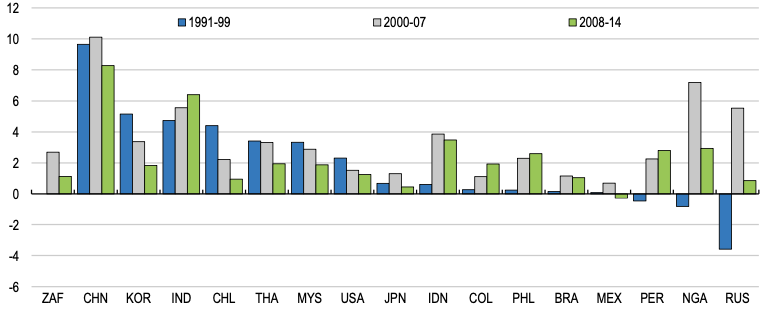
\includegraphics[scale=.3]{pic/tpin1.4.png}
        \caption{노동생산성의 연평균 성장률}
    \end{figure}
\end{frame}
%------------------------------------------------

\subsubsection{ 급속한 기술 변화의 완전한 효과는 아직 노동 생산성 증가로 반영되지 않음}

\begin{frame}{}
    \begin{itemize}
        \item 총노동생산성 증가율 둔화는 역설적으로 지속적인 기술 변화를 배경으로 발생.
        \item 빠른 기술 발전의 완전한 효과가 아직 총체적인 생산성 증가에 가시적인 영향을 주지 못할 수 있음을 시사.
    \end{itemize}
\end{frame}
%------------------------------------------------

\subsection{확산 체제의 고장}

\subsubsection{ 생산성 성과의 기업 간 격차 증가는 빠른 기술 향상과 동시에 발생하는 느린 총 노동 생산성 성장의 역설의 요인}


\begin{frame}{}
    \begin{itemize}
        \item 2000년대 초반 이후 생산성 성과의 총체적인 둔화 뒤에는 세계 최고 기업과 다른 기업의 생산성 성과 사이에 현저한 차이가 존재.
    \end{itemize}
    \begin{figure}
        \centering
        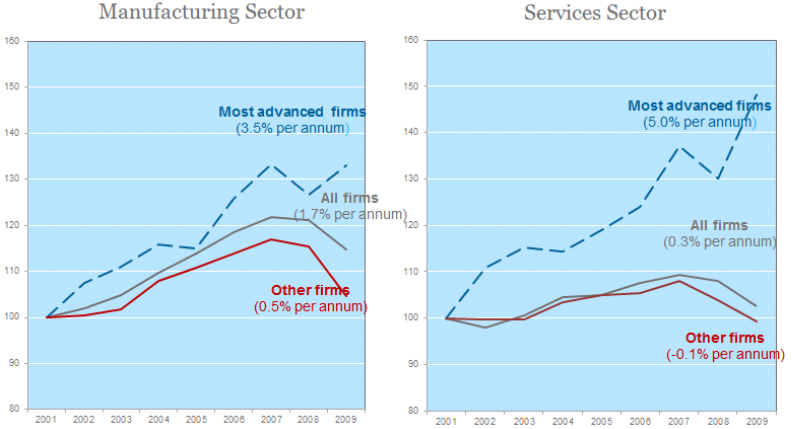
\includegraphics[scale=.3]{pic/tpin1.5.png}
        \caption{}
    \end{figure}
\end{frame}
%------------------------------------------------

\begin{frame}{}
    \begin{itemize}
        \item 일부 국가의 경우 국가 내 생산성 분포에서 여러 기업 간의 생산성 증가 차이가 발견.
        \item 이러한 생산성 격차의 원인은 국가마다 상이.
        \begin{itemize}
            \item 캐나다에서는 주로 2000년대 초에 선도기업의 생산성 폭증에서 발생.
            \item  대조적으로, 덴마크, 스웨덴은 생산성 증가에서 탈락하는 후진 기업의 문제.
            \item  대부분의 경우 생산성 격차의 증가는 선도기업과 한계기업 양쪽 모두에서 발생. (일본, 노르웨이, 스웨덴의 제조업과 프랑스와 일본의 서비스업.)
        \end{itemize}
    \end{itemize}
\end{frame}
%------------------------------------------------
\subsubsection{ 기업 간 격차 증가에 대한 몇 가지 해석}

\begin{frame}{ 기업 간 격차 증가에 대한 몇 가지 해석}
    \begin{itemize}
        \item 다른 기업들이 선도기업에서 배울 수 있는 능력이 감소.
        \item 확산 체제의 고장.
    \end{itemize}
\end{frame}
%------------------------------------------------

\begin{frame}{}
    \begin{itemize}
        \item 혁신의 속도와 선도기업의 생산성 향상은 모두 강한 상태를 유지.
        \item 기업 전략은 또한 높은 생산성 향상을 달성하는 데 중요한 역할.
        \item 다수의 기업은 새로운 기술과 모범 사례를 성공적으로 채택하는 데 실패.
    \end{itemize}
    \begin{figure}
        \centering
        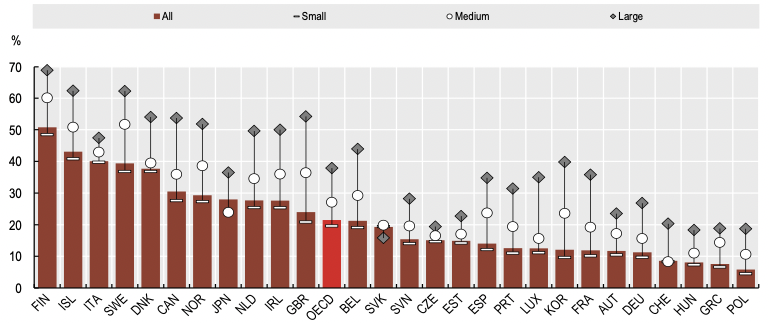
\includegraphics[scale=.3]{pic/tpin1.7.png}
        \caption{기업 규모별 클라우드 컴퓨팅 도입 비율}
    \end{figure}
\end{frame}
%------------------------------------------------

\begin{frame}{}
    \begin{itemize}
        \item 생산성 성과의 차이에 대한 다른 설명으로는 선도기업들의 지대 추구가 있으며, 이 경우 선도기업의 생산성은 더 높게 측정됨.
        \item 경제구조 자체가 선도기업들의 지대 추구에 유리할 가능 성.
    \end{itemize}
\end{frame}
%------------------------------------------------

\begin{frame}{}
    \begin{itemize}
        \item 기존 기업에 유리한 정책 설정은 시장 집중 및 임대료 추구 과정을 강화할 수 있습니다.
    \end{itemize}
    \begin{figure}
        \centering
        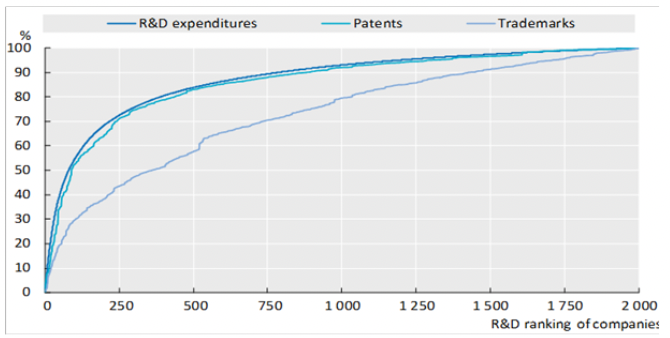
\includegraphics[scale=.3]{pic/tpin1.8.png}
        \caption{2000개 R\&D 기업의 R\&D 지출 및 지재권 누적분포}
    \end{figure}
\end{frame}
%------------------------------------------------

\begin{frame}{}
    \begin{itemize}
        \item 생산성 성장의 증가하는 격차에 대한 세 번째 보완적인 설명은 후발기업.
        \item 미래의 생산성 증가는 확산 기계의 부활로 이익을 얻는 것.
        \item 퇴장 장벽과 기술 불일치는 생산성이 낮은 활동에서 자원을 낭비하는 역할.
        \item 유사하게, 기술 불일치의 발생은 가장 생산적인 기업의 성장을 제한하기 때문에 총 생산성에 손해.
    \end{itemize}
\end{frame}
%------------------------------------------------

\subsection{ 국가 내에서 생산성 격차의 증대}

\subsubsection{ 선도지역과 낙후지역 간의 생산성 증가 격차 확대는 노동 생산성 둔화에 기여했을 수 있음}

\begin{frame}{}
    \begin{itemize}
        \item 1995년과 2013년 사이에 국가 내 지역 간 생산성 성과의 격차도 증가.
    \end{itemize}
    \begin{figure}
        \centering
        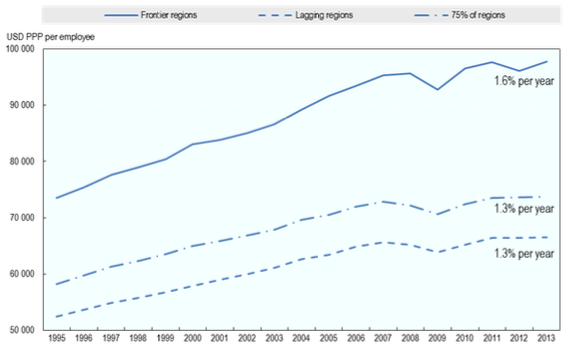
\includegraphics[scale=.3]{pic/tpin1.11.png}
        \caption{주요국의 근로자 1인당 지역별GDP}
    \end{figure}
\end{frame}
%------------------------------------------------

\begin{frame}{}
    \begin{itemize}
        \item 지역간 격차는 주로 도시-농촌간의 격차로 설명됨.
    \end{itemize}
    \begin{figure}
        \centering
        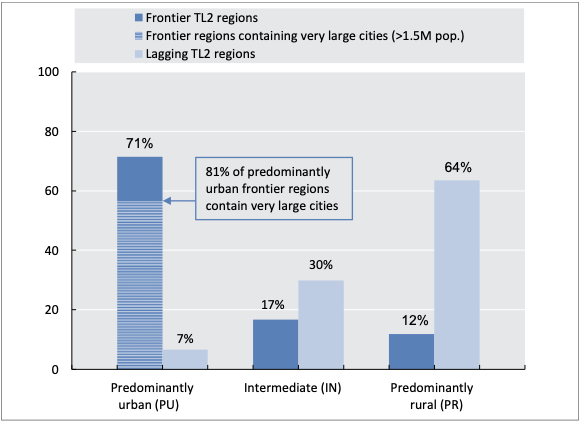
\includegraphics[scale=.3]{pic/tpin1.12.png}
        \caption{지역별 도시화율}
    \end{figure}
\end{frame}
%------------------------------------------------


\section{소득, 부, 웰빙의 불평등}

\begin{frame}{}
    \begin{itemize}
        \item 총생산성 성장률의 감소는 몇몇 OECD 국가에서 큰 부와 복지 격차와 함께 증가하는 개인 간의 소득 불평등을 배경으로 발생.
    \end{itemize}
\end{frame}
%------------------------------------------------

\subsection{소득과 부의 불평등}

\subsubsection{ 소득 불평등은 대부분의 선진국에서 증가했지만 몇몇 신흥 시장에서는 훨씬 더 높긴 했지만 최근 몇 년 동안 좁혀지는 조짐}

\begin{frame}{}
    \begin{itemize}
        \item 소득 불평등은 지난 30년 동안 대다수의 선진국에서 증가.
        \item 이는 상위 소득의 급증과 함께 하위 계층의 침체가 동시에 발생했기 때문.
    \end{itemize}
    \begin{figure}
        \centering
        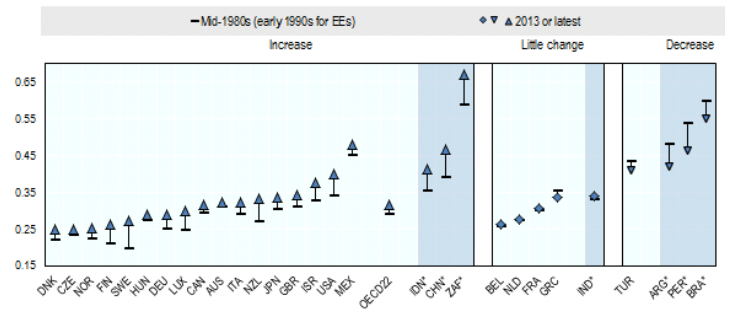
\includegraphics[scale=.3]{pic/tpin2.1.png}
        \caption{1980년대부터 2013년까지 국가별 지니계수}
    \end{figure}
\end{frame}
%------------------------------------------------

\begin{frame}{}
    \begin{itemize}
        \item 소득 분포의 확대는 소득 빈곤의 연령대의 변화를 동반.
        \item  상대적 빈곤의 위험에서 청년층이 노인층을 대체하기 시작.
    \end{itemize}
    \begin{figure}
        \centering
        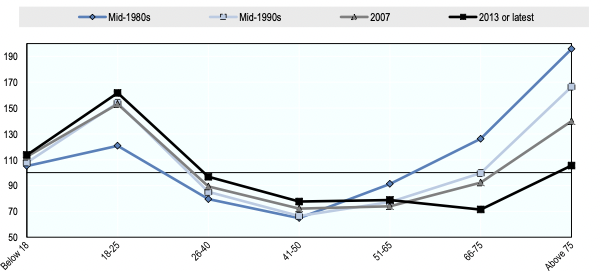
\includegraphics[scale=.3]{pic/tpin2.2.png}
        \caption{1980-2013 연령대별 상대적 빈곤률의 변화}
    \end{figure}
\end{frame}
%------------------------------------------------
\subsubsection{ 불평등의 증가는 위기와 그 여파로 인해 최하위 계층의 소득에 타격}

\begin{frame}{}
    \begin{itemize}
        \item 경제위기는 저소득층에게 가장 큰 피해를 입힘.
        \item 위기 동안 시장 소득 불평등이 심화됨에 따라 재분배 정책의 중요성이 부각.
    \end{itemize}
    \begin{figure}
        \centering
        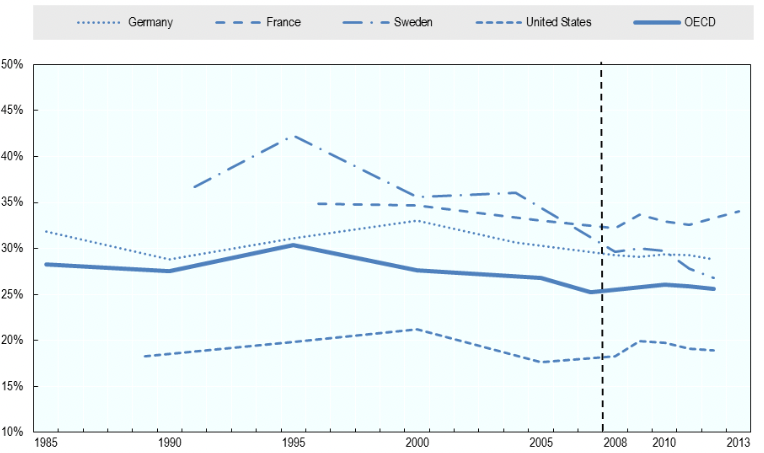
\includegraphics[scale=.3]{pic/tpin2.3.png}
        \caption{시장소득과 가처분소득으로 측정한 지니계수의 변화폭}
    \end{figure}
\end{frame}
%------------------------------------------------

\begin{frame}{}
    \begin{itemize}
        \item 전반적으로 90년대 초반 이후 대부분의 OECD 국가에서 소득 격차가 확대. 
    \end{itemize}
    \begin{figure}
        \centering
        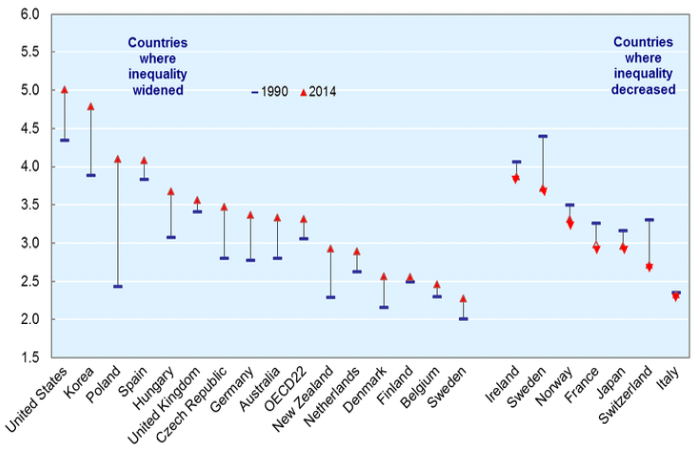
\includegraphics[scale=.3]{pic/tpin2.4.png}
        \caption{}
    \end{figure}
\end{frame}
%------------------------------------------------

\begin{frame}{}
    \begin{itemize}
        \item OECD 전체에서 부의 분배는 소득보다 훨씬 더 불평등. 
    \end{itemize}
    \begin{figure}
        \centering
        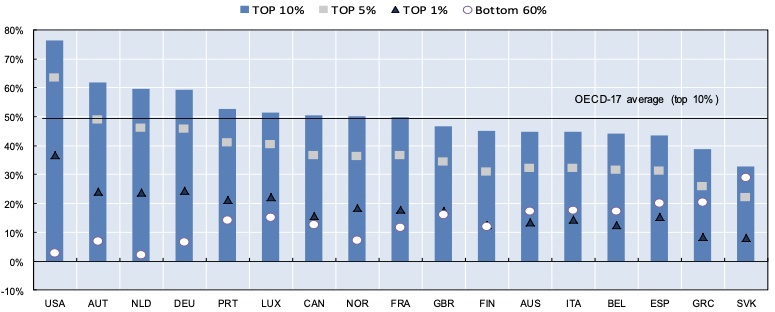
\includegraphics[scale=.3]{pic/tpin2.6.png}
        \caption{인구집단별 부의 점유 비중, 2010년}
    \end{figure}
\end{frame}
%------------------------------------------------

\begin{frame}{}
    \begin{itemize}
        \item 취업의 기회 역시 교육집단과 연령대에 따라 상이함.
    \end{itemize}
\begin{columns}
    \begin{column}{.5\textwidth}
        \begin{figure}
            \centering
            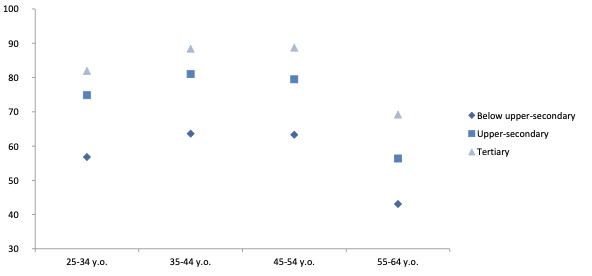
\includegraphics[scale=.3]{pic/tpin2.7a.png}
            \caption{교육집단별 연령대별 취업률}
        \end{figure}
    \end{column}    
    \begin{column}{.5\textwidth}
        \begin{figure}
            \centering
            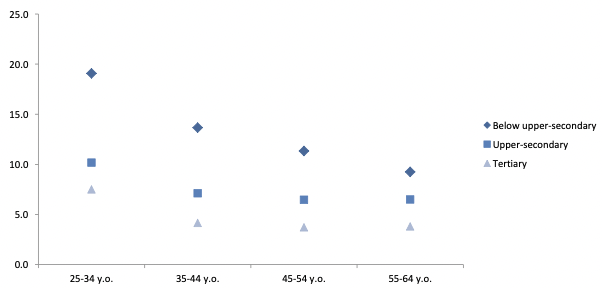
\includegraphics[scale=.3]{pic/tpin2.7.png}
            \caption{교육집단별 연령대별 실업률}
        \end{figure}
    \end{column}    
\end{columns}
\end{frame}
%------------------------------------------------

\begin{frame}{}
    \begin{itemize}
        \item 일자리와 임금의 양극화, 기술직 및 단순직 기반 기술 변화의 영향은 저숙련 및 저임금 근로자의 경제적 불안을 증가시킬 가능성이 존재.
    \end{itemize}
    \begin{figure}
        \centering
        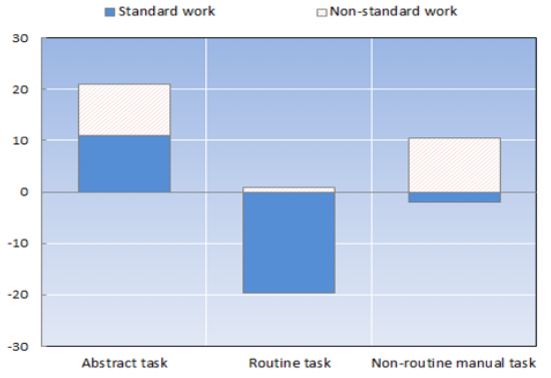
\includegraphics[scale=.3]{pic/tpin2.8.png}
        \caption{직업별 고용비중의 변화, 1995-2015}
    \end{figure}
\end{frame}
%------------------------------------------------

\begin{frame}{}
    \begin{itemize}
        \item 건강은 사람들의 생산성, 소득 및 웰빙에 중요한 영향을 미치기 때문에 건강의 불평등은 여타 요소의 불평등을 심화시킬 가능성이 존재.
    \end{itemize}
    \begin{figure}
        \centering
        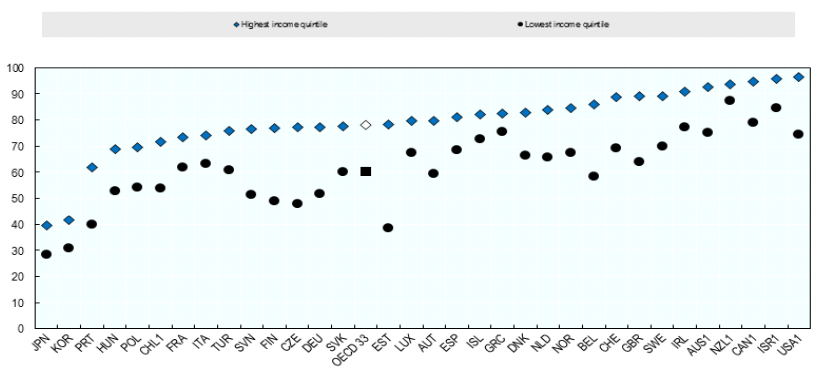
\includegraphics[scale=.3]{pic/tpin2.9.png}
        \caption{}
    \end{figure}
\end{frame}
%------------------------------------------------

\section{생산성과 불평등의 관계}

\subsection{ 불평등이 생산성과 성장에 주는 영향}

\begin{frame}{}
    \begin{itemize}
        \item 불평등의 심화와 장기적 성장 둔화가 저소득 가정의 고용 기회와 인적 자본 축적에 부정적인 영향을 미치.
        \item 이러한 세대 간 효과는 악순환을 지속적으로 만듦.
    \end{itemize}
    \begin{figure}
        \centering
        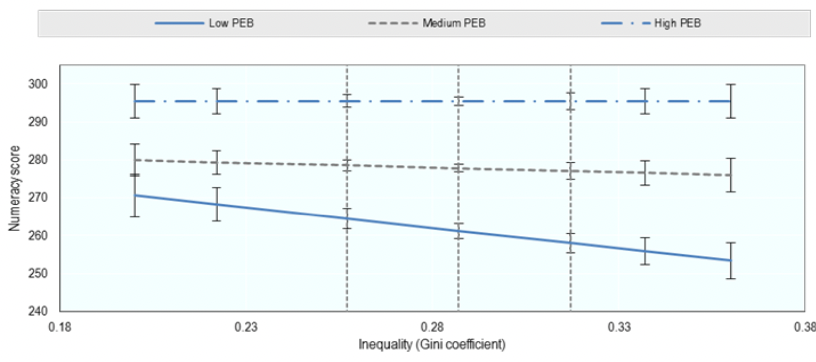
\includegraphics[scale=.3]{pic/tpin3.1.png}
        \caption{부모의 교육수준별 계산능력과 지니계수}
    \end{figure}
\end{frame}
%------------------------------------------------


\subsection{ 기술 변화, 생산성 및 불평등}

\begin{frame}{지속적인 정보 격차}
    \begin{itemize}
        \item  ICT에 대한 접근성 부족과 함께 적절한 기술의 부족은 사람들 사이의 정보 격차가 지속될 수 있음을 의미.
        \item 개인의 경우 디지털 기술에 대한 접근성이 크게 증가했지만, ICT를 효과적으로 사용하고 관련 임금 인상을 주도하는 기술은 모두에게 개방되지 않음.
        \item 같은 맥락에서 소규모 기업은 ICT 및 KBC 활용도 뒤쳐져 선도기업 생산성의 확산 지연에 기여.
        \item 지역적으로도 연결이 덜 된 기업은 형평성과 성장 측면에서 불리함.
    \end{itemize}
\end{frame}
%------------------------------------------------


\begin{frame}{디지털화와 양극화}
    \begin{itemize}
         \item 노동 수요가 고도의 추상적 기술과 저도의 수동적 기술의 두 가지 극단에서 양극화되고 있으며 중간 수준의 일상적인 기술이 필요한 직업은 진공화 되고 있음.
         \item 이러한 추세가 얼마나 멀리 그리고 빠르게 더 발전할 수 있느냐 하는 것 문제.
         \item 인공지능, 빅데이터 등의 지속적인 기술변화는 과거보다 더 극적인 변화, 특히 고용과 임금의 공백을 더욱 심화시킬 수 있음.
         \item 동시에 이러한 혁신은 더 강력한 생산성 성장과 아직 상상조차 하지 못한 새로운 일자리 역시 창출 가능.
    \end{itemize}
\end{frame}
%------------------------------------------------

\begin{frame}{지대와 승자독식}
    \begin{itemize}
        \item  앞서 논의된 생산성 성장의 둔화는 기술 변화의 특성과 기업과 정책이 상호 작용하는 방식으로 인해 악화될 수 있음.
         \item 네트워크 외부성(자연적 독점의 일종)으로 특징지어지는 부문에서 기술선도기업은 후발주자에게 기술 발전을 거의 전파하지 않고도 지속적인 경쟁 우위를 확보.
         \item 따라서 일부 선도기업은 시간이 지남에 따라 경쟁하지 않으면 생산성 확산에 부정적인 영향을 미칠 수 있는 더 많은 초과 수익(지대)를 획득가능.
         \item 이들은 직원들에게 지속적으로 더 높은 임금을 지불할 수 있게 되어 개인 수준의 불평등을 확대하는 데 기여.
         \item 해당 이론에 대한 실증적 연구가 필요.
    \end{itemize}
\end{frame}
%------------------------------------------------

\end{document}